%%%%%%%%Anhang%%%%%Anhang%%%%%%%%
%\pagenumbering{Roman}
%\pagenumbering{gobble}
\appendix

\section{Appendix}
%\subsection{Anhang A1}\label{sec:A1}
%\includepdf[pages=-]{Anhang/NE177_Requirements.pdf}
\subsection{Malware-Angriffe auf Automatisierungssysteme}\label{sec:A_Malware_Tabelle}


%\begin{landscape}
\begin{table}[H]
\centering
\rotatebox{90}{
\resizebox{1\textwidth}{!}{%\begin{minipage}{2\textwidth}%
\begin{tabular}{|l|l|l|l|l|c|}
\hline
 \rowcolor{FireBrick!80}
\textbf{Jahr} & \textbf{Ort} &\textbf{ Malware/Name} & \textbf{Details des Events} & \textbf{Angriffsart} & \textbf{Literatur} \\ \hline
2010 & Iran & Stuxnet & \begin{tabular}[c]{@{}l@{}}Infiltration von Programmier-\\ geräten (PG) und Zerstörung \\ von Zentrifugen durch \\ Steuerungsmanipulation\end{tabular} & \begin{tabular}[c]{@{}l@{}}Infiltration von PGs über infizierte\\ USB-Sticks, Injektion von schad-\\ haftem Step7 Funktionscode in \\ Siemens S7-300 Steuerungen und \\ Manipulation der Kommunikation \\ mit den Zentrifugen\end{tabular} & \cite{Symantec_Stuxnet} \\ \hline
2015/2016 & Ukraine & \begin{tabular}[c]{@{}l@{}}Crashoverride/\\ Industroyer\end{tabular} & \begin{tabular}[c]{@{}l@{}}Blackout durch einen Denial-\\ of-Service-Angriff auf Steuer-\\ ungen und SCADA-Systeme\end{tabular} & \begin{tabular}[c]{@{}l@{}}Angriff auf SPS- und SCADA-\\ Systeme des Übertragungs-\\ netzes mit den OT-Protokollen \\ IEC-101, IEC-104, IEC-61850 \\ und OPC-DA\end{tabular} & \cite{Cashoverride_Dragos} \\ \hline
2017 & Mittlerer Osten & Triton/TRISIS & \begin{tabular}[c]{@{}l@{}}Versuchte Remote-Übernahme\\ der Steuerung einer petro-\\ chemischen Anlage\end{tabular} & \begin{tabular}[c]{@{}l@{}}Angriff auf Schneider Electric \\ Triconex Sicherheitssysteme\\ (Safety Instrumented Systems,\\ SIS) und Injektion von schad-\\ haftem Steuerungscode (KOP)\end{tabular} & \cite{TRISIS_Dragos} \\ \hline
2022 & Ukraine & \begin{tabular}[c]{@{}l@{}}Industroyer2 + \\ INCONTROLLER/\\ PIPEDREAM\end{tabular} & \begin{tabular}[c]{@{}l@{}}Versuchter DoS-Angriff auf \\ das Energienetz und System-\\ Infiltration über unsicheres \\ OT-Equipment\end{tabular} & \begin{tabular}[c]{@{}l@{}}Angriff auf SPS/SCADA über \\ das IEC-104 OT-Protokoll,\\  Infiltration von OT-Kom-\\ ponenten (Siemens, Schneider \\ Electric, Omron, etc.) über \\ Netzwerk-Protokolle wie OPC\\ UA, MODBUS, CODESYS,\\ Machine Expert und Omron \\ FINS\end{tabular} & \cite{Industroyer2_forescout} \\ \hline
2022 &  & PIPEDREAM & \begin{tabular}[c]{@{}l@{}}Entdeckung der ICS-Malware\\ PIPEDREAM\end{tabular} & \begin{tabular}[c]{@{}l@{}}Infiltration von IT- und OT-\\ Netzwerken, Manipulation \\ von OPC UA Servern sowie \\ Steuerungen von Omron und \\ Schneider Electric über \\ MODBUS und CODESYS-\\ Schnittstellen\end{tabular} & \cite{Pipedream_Dragos} \\ \hline
\end{tabular}%
%\caption{Übersicht identifizierter Malware-Angriffe auf OT-Systeme in den vergangenen Jahren.}
%\end{minipage}
}}
\caption{Übersicht identifizierter Malware-Angriffe auf OT-Systeme in den vergangenen Jahren.}
%}
\label{tab:Tabelle_1}
%}
\end{table}
%\end{landscape}

\clearpage

\subsection{XML-Konfigurationsdatei}\label{sec:A1}
\subsubsection{Auzug aus einer XML}
\begin{lstlisting}[language=XML, frame=single, caption={Lorem ipsum.}, label={lst:xml-label}, captionpos=b]
<?xml version="1.0" encoding="UTF-8"?>
<opcua-servers xmlns:xsi="http://www.w3.org/2001/XMLSchema-instance"
               xsi:noNamespaceSchemaLocation="opcua-endpoints.xsd">

  <server>
    <server_app_uri>opc.tcp://172.16.4.52:4840</server_app_uri>
    <client_app_uri>urn:omag:demonstrator</client_app_uri>
    <alias>unsecured-revpi-opcua-server</alias>
    <security>
      <policy>SecurityPolicyNone</policy>
      <mode>None</mode>
    </security>
    <nodes>
      <node>
        <DisplayName>Produzierte_Takte</DisplayName>
        <NamespaceIndex>3</NamespaceIndex>
        <IdentifierType>Numeric</IdentifierType>
        <Identifier>9</Identifier>
        <datatype>String</datatype>
        <description>Names of available files</description>
      </node>
    </nodes>
  </server>
  
</opcua-servers>
\end{lstlisting}
\newpage

\subsection{Secure IoT Gateway in der Digitalen Fabrik}\label{sec:A_Demonstrator}
\begin{figure}[H]
    \centering
    \savebox{\savefig}{
\includegraphics[width=1.35\linewidth]{Figures/Platzhalter.png}}
    \rotatebox{90}{%
        \begin{minipage}{\wd\savefig}
            \usebox{\savefig}
            \caption{Lorem ipsum ...}
            \label{fig:Anhang_Demonstrator_Topview}
        \end{minipage}}
\end{figure}

\begin{figure}[H]
    \centering
    \savebox{\savefig}{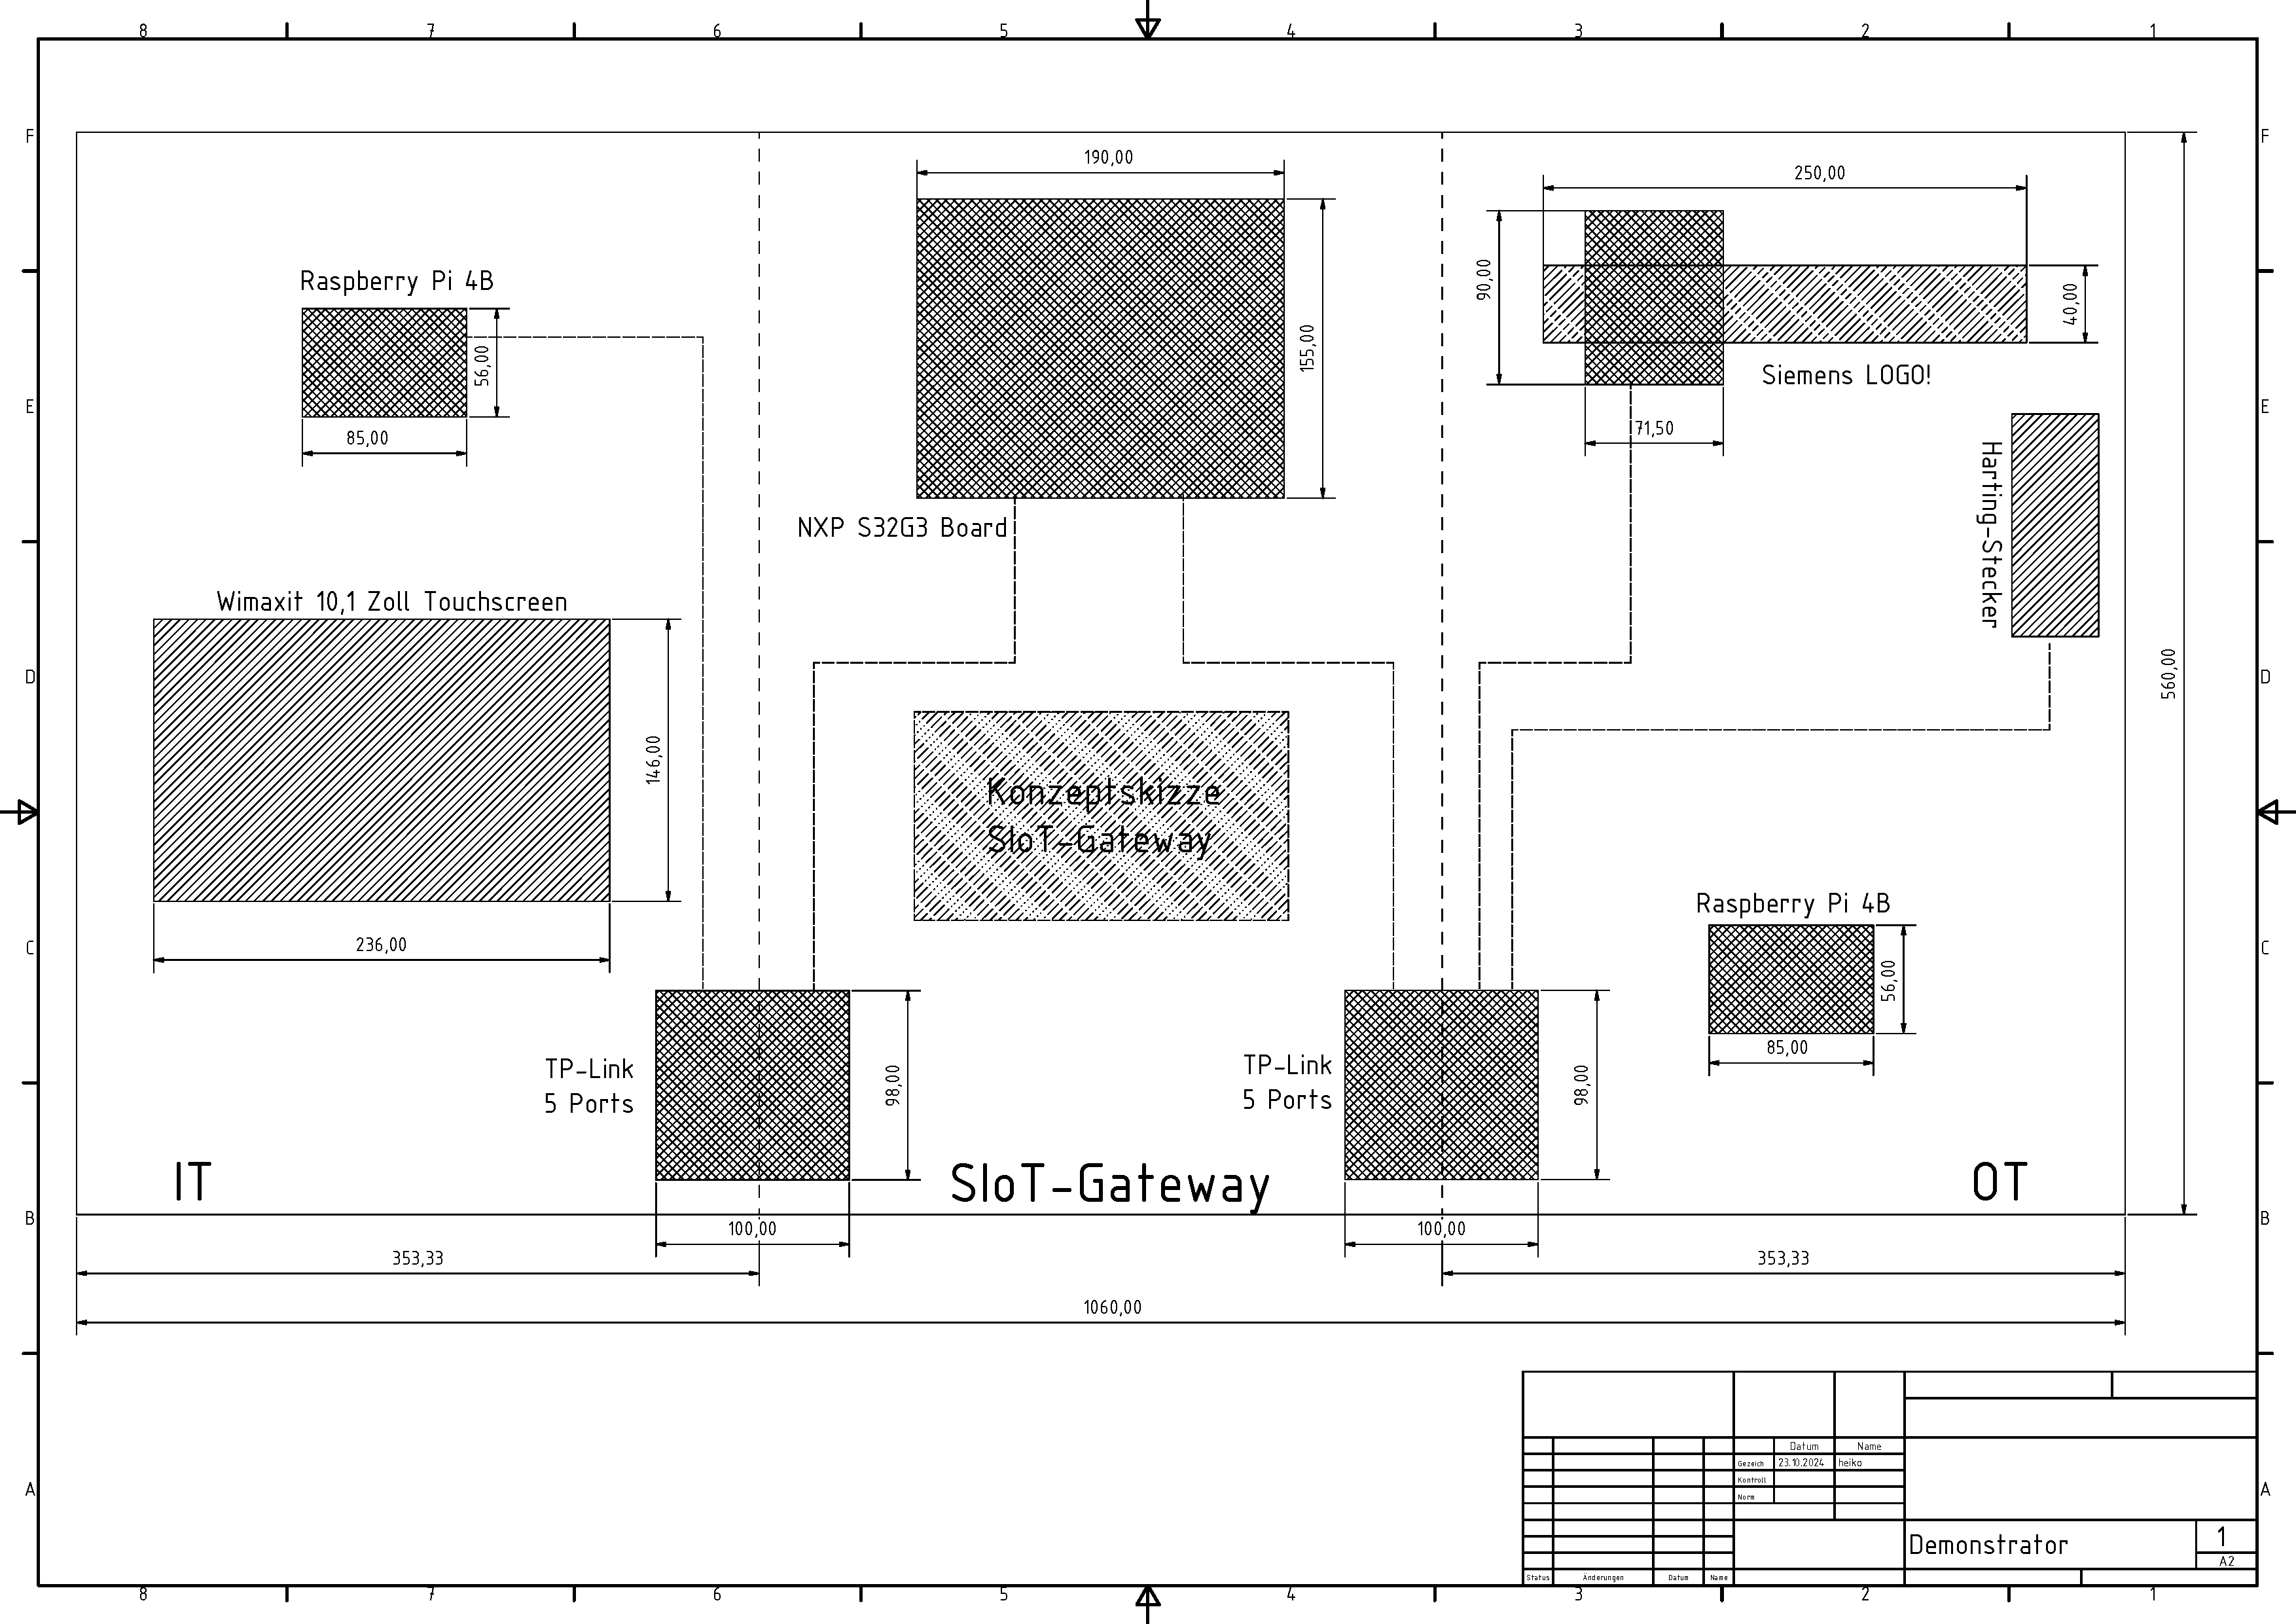
\includegraphics[width=1.3\linewidth]{Anhang/Demonstrator.pdf}}
    \rotatebox{90}{%
        \begin{minipage}{\wd\savefig}
            \usebox{\savefig}
            \caption{Lorem ipsum... (vgl. Abb. \ref{fig:Anhang_Demonstrator_Topview}).}
            \label{fig:Demonstrator}
        \end{minipage}}
\end{figure}
\newpage

%\subsection{A1}\label{sec:A1}
% ...
%\includepdf[pages=-]{Anhang/Angebot_Harting_Stecker.pdf}

%\subsection{A2}\label{sec:A2}
% ...
%\includepdf[pages=-]{Anhang/Dokumentation_Harting-Industriestecker.pdf}